% THIS IS SIGPROC-SP.TEX - VERSION 3.1
% WORKS WITH V3.2SP OF ACM_PROC_ARTICLE-SP.CLS
% APRIL 2009
%
% It is an example file showing how to use the 'acm_proc_article-sp.cls' V3.2SP
% LaTeX2e document class file for Conference Proceedings submissions.
% ----------------------------------------------------------------------------------------------------------------
% This .tex file (and associated .cls V3.2SP) *DOES NOT* produce:
%       1) The Permission Statement
%       2) The Conference (location) Info information
%       3) The Copyright Line with ACM data
%       4) Page numbering
% ---------------------------------------------------------------------------------------------------------------
% It is an example which *does* use the .bib file (from which the .bbl file
% is produced).
% REMEMBER HOWEVER: After having produced the .bbl file,
% and prior to final submission,
% you need to 'insert'  your .bbl file into your source .tex file so as to provide
% ONE 'self-contained' source file.
%
% Questions regarding SIGS should be sent to
% Adrienne Griscti ---> griscti@acm.org
%
% Questions/suggestions regarding the guidelines, .tex and .cls files, etc. to
% Gerald Murray ---> murray@hq.acm.org
%
% For tracking purposes - this is V3.1SP - APRIL 2009

\documentclass{acm_proc_article-sp}

\begin{document}

% set the path for graphics
\graphicspath{{figures/}}

\title{Continuous Transparent Authentication with User-Device Physical Unclonable Functions (UD-PUFs) based on Mobile Device Touchscreen Interactions}
%\subtitle{[Extended Abstract]
%\titlenote{A full version of this paper is available as
%\textit{Author's Guide to Preparing ACM SIG Proceedings Using
%\LaTeX$2_\epsilon$\ and BibTeX} at
%\texttt{www.acm.org/eaddress.htm}}}
%
% You need the command \numberofauthors to handle the 'placement
% and alignment' of the authors beneath the title.
%
% For aesthetic reasons, we recommend 'three authors at a time'
% i.e. three 'name/affiliation blocks' be placed beneath the title.
%
% NOTE: You are NOT restricted in how many 'rows' of
% "name/affiliations" may appear. We just ask that you restrict
% the number of 'columns' to three.
%
% Because of the available 'opening page real-estate'
% we ask you to refrain from putting more than six authors
% (two rows with three columns) beneath the article title.
% More than six makes the first-page appear very cluttered indeed.
%
% Use the \alignauthor commands to handle the names
% and affiliations for an 'aesthetic maximum' of six authors.
% Add names, affiliations, addresses for
% the seventh etc. author(s) as the argument for the
% \additionalauthors command.
% These 'additional authors' will be output/set for you
% without further effort on your part as the last section in
% the body of your article BEFORE References or any Appendices.

\numberofauthors{3} %  in this sample file, there are a *total*
% of EIGHT authors. SIX appear on the 'first-page' (for formatting
% reasons) and the remaining two appear in the \additionalauthors section.
%
\author{
% 1st. author
\alignauthor Timothy M. Dee\\
       \affaddr{Electrical \& Computer Engineering}\\
       \affaddr{Iowa State University}\\
       \affaddr{Ames, IA, USA}\\
       \email{deetimothy33@gmail.com}
% 2nd. author
\alignauthor Ian T. Richardson\\
      \affaddr{Electrical \& Computer Engineering}\\
      \affaddr{Iowa State University}\\
      \affaddr{Ames, IA, USA}\\
      \email{ian.t.rich@gmail.com}
% 3nd. author
\alignauthor Akhilesh Tyagi\\
      \affaddr{Electrical \& Computer Engineering}\\
      \affaddr{Iowa State University}\\
       \affaddr{Ames, IA, USA}\\
       \email{tyagi@iastate.edu}
}

%\date{30 July 1999}
% Just remember to make sure that the TOTAL number of authors
% is the number that will appear on the first page PLUS the
% number that will appear in the \additionalauthors section.

\maketitle
\begin{abstract}
%TODO remove the last sentence, mabe? Also, include numbers describing important results
A mobile device user continually interacts with many sensors through the natural
user interface (UI) of apps. These interactions are unique for each (user, device) pair
forming a user-device biometric.  
A physical unclonable function (PUF) can be realized
from the touch screen pressure variability. We illustrate how a sequence of these pressure values from discrete touchscreen interactions may be used to uniquely characterize a user-device pair. These
touch screen interactions Markov models can be integrated into a
continuous authentication layer. Based on the most recent sequence of touch screen
interactions, the continuous authentication layer can assign a probability that these
interactions came from the authenticated (user, device) pair. Continuous authentication may help protect access to a mobile device from a malicious party by detecting the
anomalies early. The effectiveness of this scheme is described in terms of how definitively can one user  be differentiated from another.
\end{abstract}

% A category with the (minimum) three required fields
%\category{H.4}{Information Systems Applications}{Miscellaneous}
%A category including the fourth, optional field follows...
%\category{D.2.8}{Software Engineering}{Metrics}[complexity measures, performance measures]

%\terms{Theory}

%\keywords{physical unclonable function (PUF), user device physical unclonable function (UD-PUF)} % NOT required for Proceedings

\section{Introduction}
\label{sec:intro}
%Motivate the reasoning behind why we may want to secure mobile devices more
Mobile devices are ubiquitous in the modern world. These devices are becoming progressively more important for many applications with hold sensitive data such as financial and health care data. 
Securing mobile devices poses unique challenges and opportunities. Traditional user authentication
is a single challenge-response model based on a password. 
 A mobile device, however, has a greater number of available device sensors that have been
used to capture the uniqueness of a specific user, device interaction for enhanced traditional
user authentication. Traditional user authentication however leaves large gaps in between successive
user authentications. If the device is compromised in between two successive user authentications,
there is a long time available to the adversary for inflicting damage. This paper proposes a
continuous authentication framework in which an authentication framework running in the background 
is continually monitoring user activities. Moreover, this monitoring is based on the 
combined biometric of the user and the device silicon captured as a physical unclonable function (PUF).
%

%develop an understanding of the need for this system
 Traditional physical unclonable functions (PUFs) which generate a unique signature of a given hardware device are not sufficient to guarantee the identity of a user.
A mechanism that combines the biometric identity of a human user and the device silicon in 
a way that is not mathematically separable is more robust in the mobile world. UD-PUFs (user-device
entangled physical unclonable functions) \cite{ScheelTyagi15} serve just that role.
Integration of such UD-PUFs into a continuous authentication environment is the main problem
addressed in this paper.


%problem statement, describe what the UD-PUF must accomplish 
A UD-PUF is a function of both the device silicon and the user behavior. Such a function must show 
significant change in the output given a small change in any component of a user-device pair
somewhat like a hash function. Hence the UD-PUF must be based on a property or properties which vary significantly and identifiably among mobile device hardware and users. The best candidates to use will be properties which offer the most variability, and properties which are most easily exposed in the android operating system.

%problem statement continued, what must be the properties of the authentication system.
System efficiency and response times imposes additional constraints on properties to base a UD-PUF on.
The system must also be practical under normal use conditions for mobile devices. The system must be non-intrusive to the user, fast enough to run on mobile devices, and accurate when authenticating users. If a user must spend a long time authenticating they are not able to use this time to accomplish the task for which they are being authenticated. This detracts from the efficiency of using a mobile device to complete the task. If the proposed system is too computationally intensive to be run on a mobile device, or the system has low accuracy then it is useless for any practical application. 
%For these reasons we propose a system which operates under a continuous authentication scheme.

%describe in depth the continuous authentication scheme proposed, this is where the main contributions of this work should be discussed
In the continuation authentication world, a composite sensor vector \cite{zhu2013sensec} has been used
to establish a user identity. Other user biometrics such as inter key stroke timing have also been
used. In this paper, the continuous authentication is based on a combined user-device identity.
The continuous authentication signature will fail if either the biometrically correct human being
or the biometrically correct device component is removed.
 This paper builds the continuous authentication framework on the user touch screen interactions.
We establish that the user touch screen interactions do differentiate one user from another. 
Note that there are advantages to basing a framework on a single source of information. A failure of the touchscreen to function also constitutes device failure. This system is more robust because it will only fail upon failure of the device touch screen. Compare this to other systems whose functionality depends on many components. A failure in any one of these components disrupts the authentication scheme making these systems more prone to failure. 


Continuous authentication frameworks' basis premise is that a user behavior over time gravitates
towards  predictable. It can be frequently modeled as an $n$-Markov model. It states that the
user tokens of length $n$ repeat themselves with certain frequency. Hence if we can record history
of $n$-token sequences, they could help us classify the user's current behavior. The tokens are
touch screen pressure values that are continually generated as the user interacts with an app
through a soft keyboard.


%benefit of continuious authentication over other systems
Consider an authentication scheme which seeks to achieve authentication over the duration of a device's use, but requires that some action must actively be taken by the user. Say that this system requires the user to complete some gesture in response to an image on the screen.
This sort of authentication my interupt the user durring important tasks, or otherwise cause the device to be more difficult to use.
This may lead to great frustration on the part of the user at having to reauthenticate.
This senerio exposes a clear benefit of continious authentication which runs in the background. If the authentication system utilizes actions which are already being preformed by the user to preform the authentication then the user can go about their business completly unaware and uninterupted by the authentication system. 
This means additional security is possible without causing undo stress on the user or making interation with the device an unpleasent experience.


% describe the structure of the paper, what is contained in each section
The structure of the paper is as follows. Section \ref{sec:related_work} discusses related work. Touchscreen pressure and the corresponding UD-PUF model are described in section \ref{sec:touchscreen}. The $n$-Markov model and its parametrization are discussed in section \ref{sec:modeling}. 
%Section \ref{touch_pressure_modeling} provides some implementation details with respect to how touchscreen pressure is used in the modeling scheme. 
Data collection methods are discussed in section \ref{sec:data_collection}. The authentication scheme is discussed in section \ref{sec:differentiation}. The results including final numbers and suggestions in practical applications are articulated in section \ref{sec:results}. Conclusions are presented in section \ref{sec:conclusions}. Finally section \ref{sec:futurework} discusses future work in this area. 

\section{Related Work}
\label{sec:related_work}
%detail what was done in the sensec paper
SenSec, a similar authentication scheme to the one proposed in this paper, completed at Carnegie Mellon used information from from accelerometers, gyroscopes and magnetometers to construct a model of a user. \cite{zhu2013sensec} This method can be classified as a UD-PUF as each accelerometer, gyroscope and magnetometer will have some variance inherent in the manufacturing process for these devices \cite{?}; the input to these devices will also vary significantly by user \cite{?}. As a result the output is a function which varies with changes in user or device, a UD-PUF.

%TODO more about sensec, relate things in sensec back to our work
%TODO explain what we can learn from sensec use of marcov chain
Another noteable aspect of the SenSec system is their method of modeling users with an $n$-Markov model. This system presents several benefits which include relative simplicity and scaleability. \cite{zhu2013sensec} 

\cite{shi2011senguard}
\cite{feng2012continuous}

%TODO provide a brief history of UD-PUFS
%TODO explain why are solution is better than previous/other solutions

%TODO describe how our work differes from that of our predecessors

%describe what touchscreen pressure is
%describe the physical component of the pressure (current at the edge of screen on android device)
\section{Touchscreen Pressure}
\label{sec:touchscreen}
%describe how touchscreens work
Many mobile devices today are equiped with capacitive touchscreens which have the ability to approximate, among other metrics, the pressure of a given interaction with the touchscreen. \cite{?} 
When a user interacts with the touchscreen of their device they typically put their finger or fingers on the screen in order to indicate what operation they want the device to preform. This contact (or near contact) functions to increase the capacitance of the screen in a predictable way. 
The touchscreen is split into many rows and columns; capacitance is measured indirectally as a function of the current increase in the row and column containing the touch.\ref{?} 

%describe what is touchscreen pressure
If our goal is be be able to distinguish a user's interaction with a given device from this same user on a different device and from different users on any device than our description of the user will need to be a product of both the user and the device. 
In the android operating system there exists a pressure function which returns a value proportional to current at sides of the touchscreen for a given touchscreen interaction. \cite{?} 
This measurement is a function of both the device silicon and the way the interacts with the touchscreen making this measurement a reasonable choice for use in our system.
This is the value which will serve as the basis for our scheme and will henseforth be referred to as touch pressure. 

%TODO describe why touchscreen pressure is a good candidate for our UD-PUF
The pressure function is significant because it's value not only depends on the characteristics of the device but also on the way in which a user interacts with a given device. The effect of a given device on the touch pressure value will differ significantly due to variations implicit in the manufacturing process for the touchscreens of these devices. \cite{manufacturing_differences} Our supposition is a given user will interact with a touchscreen in such a way as to cause significant variations in the touch pressure values when compared to other users on the same touchscreen \cite{user_touchscreen_interations}.  Given this, we have chosen touch pressure as the basis for our UD-PUF.

%TODO describe how we use touch pressure in our system, modeling and authentication
In our system, we reccord the touch pressures generated by the user when they are using the system's soft keyboard. Once we have collected a sufficient number of touches, authentications may begin to be preformed on new data. Figure \ref{fig:authentication_accuracy} demonstrates that as few as 6000-8000 touches may be used to achieve accuracies higher than 80\%.
A typical user can enter information into a devices soft keyboard at a rate of xx words per minute. \ref{}. %TODO do the calculations about how long before
A word is on average five letters long leading to a rate of xx*5 touch interations per minute.
This means in the average use case a user will generate enough information to begin being authenticated in about x minutes of continious use.
Many applications utilize this as a method of input meaning that in the average use case there will be a constant influx of new data to be analyzed.

%describe a marcov model in general
%describe what it means to be an n-gram sliding marcov model
%describe in what way we a marcov model to describe a user, device pair (our marcov model of touch, pressure values.
%An n-gram sliding marcov model.
\section{Modeling a User-Device Pair}
\label{sec:modeling}
%describe the motivation for the use of a marcov chain
Interactions between users and devices are complex. To interpret these actions in a meaningful way, in order to perform an authentication for example, it is necessary to simplify these interactions. The chosen model must provide sufficient entropy such that a model generated with a given user-device pair is not consistently reproducible by another user or on a different device. The modeling method must also be easily reproducible by the original user on the original device. A model having the necessary characteristics required for this application is a Markov Chain.

%TODO describe what is a marcov chain
Markov Chains are useful in predicting systems whose behavior can be modeled in discrete states. The transitions between states can be identified to happen with some probability.
In general an $n$-Markov model states that the
user tokens of length $n$ repeat themselves with certain frequency. Hence if we can record history
of $n$-token sequences, they could help us classify the user's current behavior. The tokens are
touch screen pressure values that are continually generated as the user interacts with an app
through a soft keyboard.

%Other information about marcov chains
%TODO traditional use of marcov chains
%Historically the Marcov Chain has found applications in (statistics?)

%begin talking about the construction of the model
Upon identification of an appropriate model the next step is to discover an optimal way in which it may be applied to the current problem. Interactions between a user and device can be described as a sequence of touch pressure values which accumulates over time
as the user continues to interact with apps though a soft keyboard.
We use $n$-sized subsets of this sequence in the $n$-Markov model constructed for the user.\cite{marcov_chains_previous_n_values}

%demonstrates how the range is split into many distinct token ranges by pressure
\begin{figure}
\centering
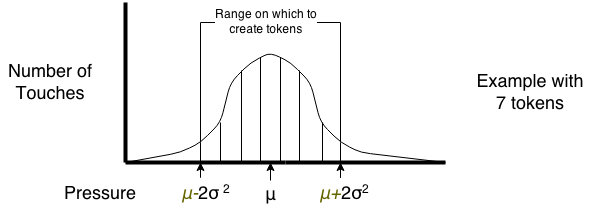
\includegraphics[width=3.9in]{token_creation.png}
\caption{Describes how a distribution may be split into distinct token ranges by pressure.}
\label{fig:token_creation}
\end{figure}

%TODO continue talking about model construction.
%how are tokens constructed
%how are probabilities calculated
In building the model we remove some touches likely to be mistakes by the user or simply outliers in the data set.
The distribution of touch pressue values is calculated for each area on the touchscreen with which the user interacts. In our system these areas correspond to keys of the soft keyboard but they are not restricted to be this.
The distribution, $\mu$ and $\sigma$, values are calculated for each of these areas.
If a key falls outside of $\mu\pm2\sigma$ for a given area, then it is not included in any of the $n$-token sequences. 
Figure \ref{fig:token_creation} illustrates how this works on a distribution which has been split into 7 token ranges.
The value of $\mu\pm2\sigma$ was chosen because statistically xx\% of touches will fall withing this range for normally distributed data. \ref{statistically_xx_percent} Figure \ref{fig:normal_distribution} plots a set of touch pressures from one of our users which shows that our data can be described as having a normal distribution.
For tokens to be considered equal, both the area from which the touch was generated and the pressure must match.

%shows that our data is normally distributed
\begin{figure}
\centering
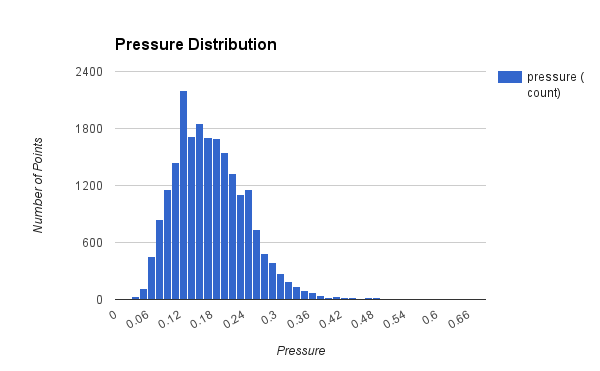
\includegraphics[width=3.9in]{normal_distribution.png}
\caption{This chart displays a set of pressure data from one of our uses. Note that the pressure values are nomally distributed.}
\label{fig:normal_distribution}
\end{figure}

%n-gram a continuious sequence of n items
%markov model for comparason is built from a sliding model of the previous n touches
%describe how the marcov chain is applied to touch pressure to model a user
%this is a description of our specific implementation of a marcov model
%\section{Touch Pressure Modeling}
%\label{touch_pressure_modeling}
% this section should describe various implementation details
%TODO it may be useful to include all different parameters to the model, and the effects of varying each of them

%describes how the marcov model is built from the sequence of touch pressures
\begin{figure*}
\centering
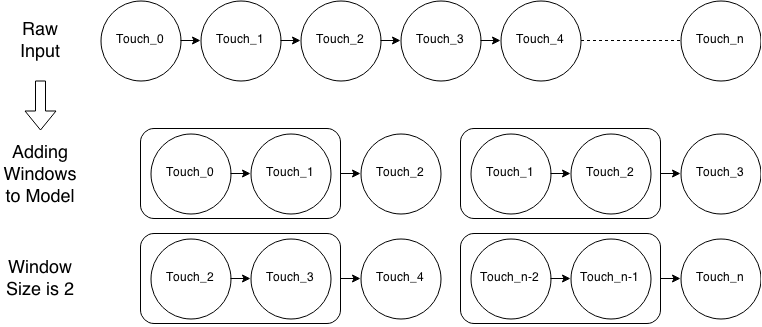
\includegraphics[width=3.9in]{marcov_model_building.png}
\caption{The top of this figure depicts the raw imput origionating from the touchscreen. Each touch represents a single interaction between the user and the human user and the soft keyboard of the mobile device. The bottom images show how the raw input is organized into the marcov model. For example, the bottom left image can be interpreted as Touch\_4 succeeds the sequence Touch\_2, Touch\_3 with some probability.}
\label{fig:markov_model_building}
\end{figure*}

%TODO desctibe, or reference somewhere, the above pictures

%TODO describe the marcov model used
The goal in modeling a system with a Markov model is to classify the system in terms of its transitions between states. If such a model is to be used to purposes of uniquely identifying a given system, than the model must be chosen in a way which exposes the uniqueness of the system. Our scheme uses a Markov model constructed from the sequence of touches entered by a user through the soft keyboard.
Each touch contains information about the pressure and location of the interaction with the touchscreen.

%TODO describe aspects of the implementation
%describe how the model is constructed from the touch pressure sequence
Our Markov model calculates the probability of a given touch coming after a sequence of $n$ touchs.
$n$ is a parameter to the model which should allow for increased accuracy in determining the true probability of a given touch to come after a preceeding sequence of touches when given more data to construct the model. The increased accuracy is due to a greater number of possible model states which decreases the liklihood that a user will have states which overlap a different user.
Figure \ref{fig:markov_model_building} demonstrates how the sequences for the Marcov model are generated from the user's raw input into the soft keyboard.

%describes how the marcov model will look after it has been constructed
\begin{figure*}
\centering
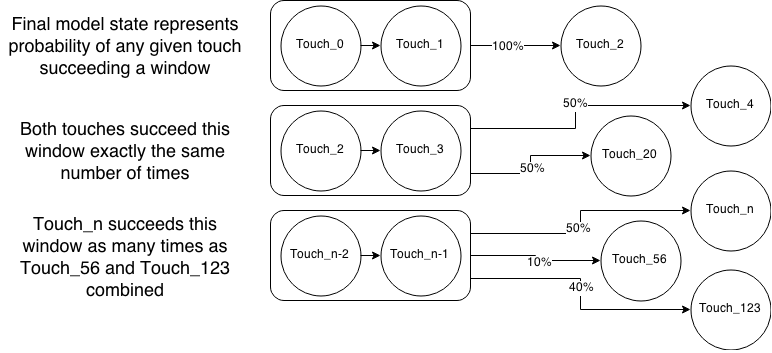
\includegraphics[width=3.9in]{final_marcov_model_state.png}
\caption{This figure depicts the state of the Markov model after the probabilities have been calculated. The top image, for example, may be interpreted as Touch\_2 succeeds the sequence Touch\_0, Touch\_1 with probability 100\%.}
\label{fig:final_markov_model_state}
\end{figure*}

%TODO describe the probability calculation in detail
The probability of a touch coming after a sequence of touches can be expressed as the number of occurrences of touch after a given sequence by the total number of occurrences of that sequence.
The idea behind this probability calculation is illustrated in Figure \ref{fig:final_markov_model_state}.
Noteably, Touch\_$n$ is not distinct. In other words Touch\_$a$ will be considered equal to Touch\_$b$ if the keycodes of these touches are equal and the touches fall within the same pressure range. Pressure ranges are depicted in Figure \ref{fig:token_creation}.

%TODO talk about how prefix tree is used to store these sequences in order to increase the speed.
%TODO cite some source which supports the benefits of a prefix tree
%TODO explain what a prefix tree is
%TODO include some figures to illustrate what a prefix tree is
The information needed to calculate the probability of a touch succeeding a given sequence is the number of times that touch succeeds the sequence and the number of times the sequence occurrs.
The use of a prefix tree as a data structure can be used to make both of these numbers more readily accessible thus increasing the speed of the probability calculation.
%TODO explain how prefix tree makes them readily accessible

%TODO explain why this increases the speed of the probability caluclation... articulate how an alternative data structure would perform


%explain how the prefix tree is implemented in our system
In our system the $n$-token sequences are stored in a list while a prefix tree is used to store information about the each sequence.
This information is stored on the nodes of the tree; it includes the number of occurrences of a sequence and a list of indexes where the sequence occurrs in the list storeing all the sequences.
This index list is useful because it eliminates the need to search the list in order to determine what the successor touches of a window are.
This approach requires much fewer calculations compared to simply using a list to store the sequences. 
If only a list is used then in order to determine how many times a sequence occurrs the list must be searched.

%TODO this is the place for MLE, maximal liklihood estimation formulas
\ref{something with mle formulas}


%basically the authentication scheme used
%frame it in more general terms, independent of our specific application
\section{Differentiating User-Device Pairs}
\label{sec:differentiation}
%TODO describe each of the model parameters in detail
%TODO state how each of the best model parameters were determined


%this figure describes how false positive and false negative percentages vary based on authentication threshold
\begin{figure}
\centering
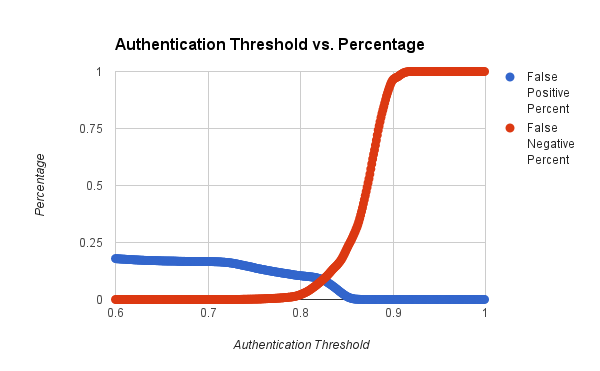
\includegraphics[width=3.9in]{threshold_vs_percentages.png}
\caption{Describes how false positive and false negative percentages vary as the authentication threshold is adjusted.}
\label{fig:threshold_vs_percentages}
\end{figure}

%TODO
%describe what the authentication threshold is
%define false positive
%define false negative
%explain why the intersection of these two is significant in choosing the authentication threshold
In distinguishing a particular user from another different user, it is necessary to develop a method of comparison between users. In our method of comparison we take the probability associated with a touch pressure coming after a sequence of preceding touch pressures for a particular user and compute the difference between this probability and the probability of the same touch pressure coming after the same sequence of touches for a different user. The average of these probability differences is taken to be the difference between two users.
%
Once a comparison is established a natural extension is a system of authentication. This system needs to determine when two sets of touch pressure values came from the same user-device pair. When authenticating a user, we take one minus the average difference between the model constructed from the two sets of touch pressure values. Take this value to be the authentication percentage for a given set of touch pressure values against another.
%
%add more metrics, and explain them, provide more graphs about them
To determine how well this system does at differentiating users it is useful to develop metrics which describe the system's performance under conditions which are similar to it's potential real-world applications. Figure \ref{fig:threshold_vs_percentages} illustrates how false positive percentage and false negative percentage vary based on where the threshold for authentication is set. 

%authentication threshold described
Here, authentication threshold refers to the value of authentication percentage one model must have against another for the models to be considered the same; two models which are the same are supposed to have been created from touches generated by the same user-device pair.
%false positive percentage described
False positive percentage measures what fraction of authentications between two sets of touch pressures which did not come from the same user-device pair, therefore these sets should not be considered the same, but did authenticate as being the same in our authentication system.
%false negative percentage described
False negative percentage is exactly the inverse of false positive percentage in that it describes what fraction of authentications between two sets of touch pressures which did come from the same user-device pair, but did not authenticate as being the same in our authentication system.

%significance of the intersection of false positive, false negative values
In Figure \ref{fig:threshold_vs_percentages} there exists a clear intersection between false negative and false positive percentages. This intersection is significant; at this point the system neither biased toward allowing user-device pairs which should not authenticate to pass authentication nor toward disallowing user-device pairs, which should authenticate, from passing authentication. This point represents a balance in design, but the best authentication threshold will depend on the application of this system.

%TODO describe the implementation of the authentication system, how the compairason works
The implementation of the authentication system is as follows. A Markov model is constructed from a sequence of touches known to have come from the user. A seperate Markov model is then constructed from a sequence of touches which need to be compaired to the model.
The model coming from the later sequence of touches is created with the same distribution as the base model. This affects the $n$-sized touches sequences which are added to the authentication model.
Sequences containing touches which fall outside the base model's distribution are thrown out.
The probabilities computed for each of these models are then compaired and a percent difference is derived from these compairasons. We then choose to authentication only those models which have achieved a low enough percent difference.

%TODO describe the model compairason
In comparing the base and auth Markov models each $n$-token sequence in the auth model is compared to the base model.
For a given sequence in the auth model the base model is searched for a matching sequence.
If a matching sequence is not found then the sequence in the auth model being considered is decided to be maximally different.
If a matching sequence is found than the absolute value of the differance between probabilities computed for that sequence are considered to be the difference.
The aggragate difference is the average of these difference values.  

\section{Data Collection and Analysis}
\label{sec:data_collection}
%TODO
%describe the number of users from which the data was collected
%describe the method of collection
Data for creating touch pressure models in this experiment was generated using a special keyboard application for the android operating system. Users would load the keyboard onto their device and continue using the device in the way they would normally. Some users were asked to play a typing game in order to help expedite the data collection process. After the users had generated at least ten thousand touches the data was collected from the user's device.
%TODO put the data in context by detailing the number of touches collected from each user and the number of touches used to build the model

%TODO describe the user base from which the data was collected for the results presented here
The results presented here were derived from the touch data generated by two users. These users each used two different devices creating four user-device pairs each having a large number of touches.
Each user was asked to use two different devices to collect data.
The size of the data sets collected were at least 4500 and at most 47500.

%TODO describe how the data was analyzed


%what number of states exposed the most uniqueness e.g. how many tokens were best
%with what accuracy could users be distinguished from one-another
\section{Results}
\label{sec:results}
%TODO discuss predictions and whether they were correct or incorrect.
We predicted that an increase in the number of touches used to build the model would provide better accuracy in authentications. 
In additon, 

%this section describes how authentication accuracy was investigated. Also included are a few figures which describe the best authentication accuracy percentage
\begin{figure}
\centering
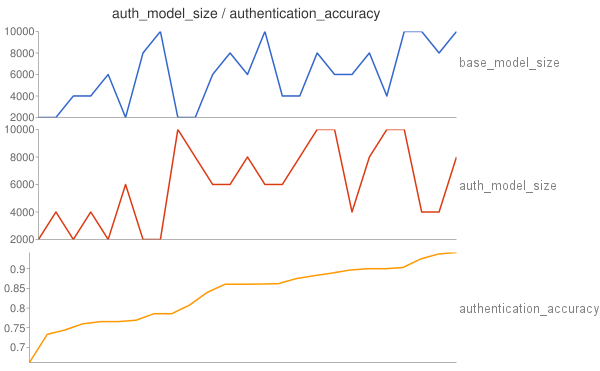
\includegraphics[width=3.9in]{authentication_accuracy_vs_model_size.png}
\caption{Authentication accuracy is a function of both the base model size and authentication model size.}
\label{fig:authentication_accuracy}
\end{figure}

%explain the contents of this figure.
%explain what each of the metrics used in the figure are.
%
In exploring the design space of this system we are trying to determine how well the system will perform in the end use case. Perhaps the best measure of the system's performance is how accurate the system is when authenticating users. Figure \ref{fig:authentication_accuracy} depicts authentication\_accuracy as a function of base\_model\_size, number of touches known to have originated from an authentic user, and auth\_model\_size, number of touches which are to be checked against the model generated from the base touches. We define authentication\_accuracy to be the percentage of authentications for which our system makes the correct decision. In other words, an authentic user is authenticated and a non-authentic user is not authenticated. The size of base model and user model which result in a given authentication accuracy are aligned with that authentication accuracy on the horizontal axis in the chart. 

%explain why more touches does not always equal more accuracy
In some instances, increased numbers of touches did not result in higher authentication accuracies. 
These lower accuracies seem to correspond to areas where %TODO
 This could be a result of the way the model decides to include $n$-sized touch sequences in the authentication. 
In this case, an auth model which is  different will authenticate with low probability because sequences are punished for not existing in the base model if they exist in the auth model.
If there are not many $n$-token sequences in the base model then high differences will be prepresent for models which are only slightly different, because many sequnces will not exist in the base model.
These sequences will be considered maximally different and constitute a high proportion of the number of $n$-token sequences.
The overall difference between two models is the average of the difference in probabilities between their $n$-token sequences; thus a high proportion of these sequences presenting a maximally different will cause the aggragate differance to be lower.
%an alternative explaination
%An alternitive explaination could be In the authentication, the distribution which was calculated for the base model is also used for the auth model.

%describes authentication accuracy dependence on the amount of user data
\begin{figure}
\centering
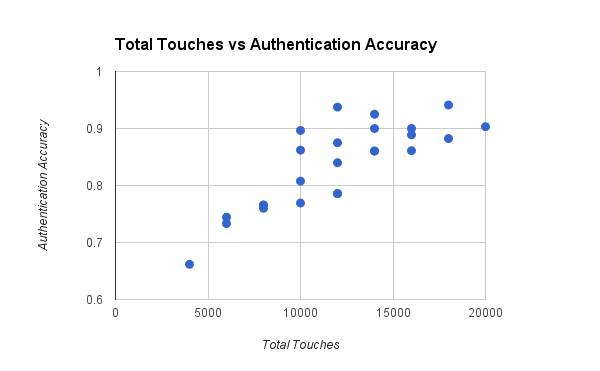
\includegraphics[width=3.9in]{total_touches_vs_authentication_accuracy.png}
\caption{Authentication accuracy is linked more closely to the total number of touches used in the authentication then to either the base model size or the authentication model size. Although authentication accuracy does not strictly increase with the number of touches it does trend upward.}
\label{fig:total_touches_vs_authentication_accuracy}
\end{figure}

%TODO explain the contents of this figure.
%explain what each of the metrics used in the figure are.
%
Figure \ref{fig:total_touches_vs_authentication_accuracy} presents the tradeoff between the amount of data needed for an authentication, and the accuracy of that authentication.
In general, more data will yeild a better authentication accuracy, but this is not always true.
The size of the base model seems to contribute more to authentication accuracy then does the size of the authentication model, therefore, if the goal is to increase authentication accuracy it seems to be better to increase the size of the base model compared to increasing the size of the authentication model.


%TODO remove, and remove all reference to this
%\begin{figure}
%\centering
%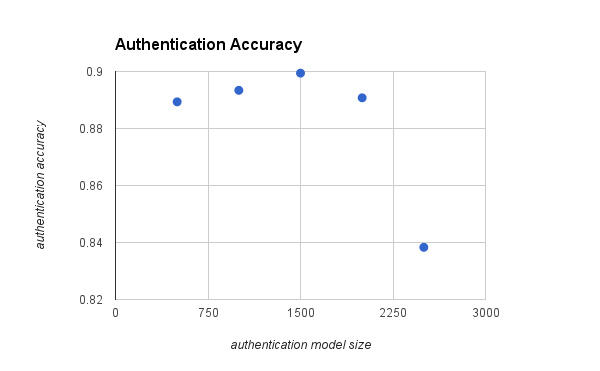
\includegraphics[width=3.9in]{extensive_authentication_accuracy.png}
%\caption{Depicts the result of many model comparisons done around the area of best results in Figure \ref{fig:authentication_accuracy}.}
%\label{fig:extensive_authentication_accuracy}
%\end{figure}

%explain the contents of this figure.
%explain what each of the metrics used in the figure are.
%
%To establish that the results in Figure \ref{fig:authentication_accuracy} hold for large numbers of comparisons many more comparisons where done around the area of best results. The results of these tests are presented in Figure \ref{fig:authentication:accuracy}. For the results depicted in the figure, user\_model\_size is held constant at ten thousand while auth\_model\_size is varied. The test was performed in this way because variations in auth\_model\_size seems to have a greater impact on authentication accuracy than variations in base\_model\_size. Approximately the same trend as seen in Figure \ref{fig:authentication_accuracy} presents itself in Figure \ref{fig:extensive_authentication_accuracy}.

\begin{figure}
\centering
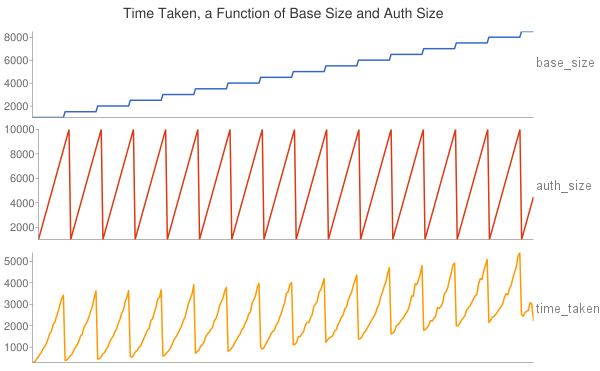
\includegraphics[width=3.9in]{nexus_speed_test.png}
\caption{Depicts the time taken on a Nexus 7 tablet as a function of base model size and auth model size. Time taken is measured in milliseconds while model sizes are measured by number of touches.}
\label{fig:nexus_speed_test}
\end{figure}

%explain the contents of these figures.
%explain what each of the metrics used in the figure are.
%fig:nexus_speed_test
Figure \ref{fig:nexus_speed_test} depicts the runtime of our system on a Nexus 7 tablet. Time taken is measured in milliseconds while model sizes are measuered by number of touches used to construct the model. 
The time taken metric does not include the overhead associated with adding touches to either the base or auth models; it is assumed this will be done over time as the user enters data. In addition, adding touches is not a computationally intense activty as it is designed to be done in constant time. 
Time taken does include the probability computation for each of the models and the compairason between the models.
This chart is a good representation of how each of the model sizes affect the runtime of the system and allows for the identification of an overall trend in the system's runtime. The overall time taken is trending upward as both base model size and auth model size increase; this suggests that the total number of touches used, that is the sum of base model size and auth model size, might be the most important factor in determining the runtime.
The dependence on the total number of touches makes sence because the majority of the computations are used to determine the probabilitys of the Marcov model. A greater number of touches in a model reqires more of these probility computations to take place.
Also of note, base model size and auth model size seem to affect time taken differently. A change of $k$ in the size of auth model seems to increase the total amount of time taken more than the same $k$-sized change in the base model. 

\begin{figure}
\centering
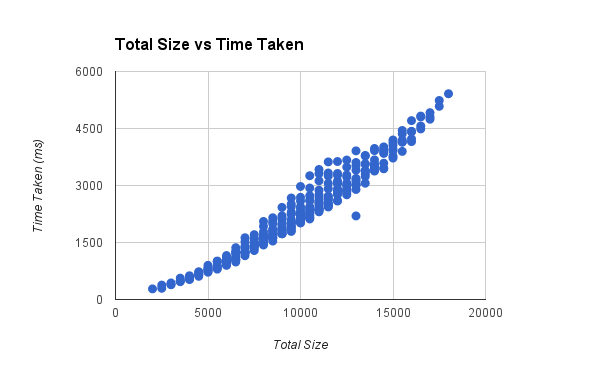
\includegraphics[width=3.9in]{nexus_total_size_time.png}
\caption{Depicts the time taken on a Nexus 7 tablet as a function of base model size plus auth model size. Time taken is measured in milliseconds while model sizes are measured by number of touches.}
\label{fig:nexus_total_size_time}
\end{figure}

%fig:nexus_total_size_time
Figure \ref{fig:nexus_total_size_time} illustrates how the time taken depends on the total number of touches used in createing the models. That is to say total size is the sum of base model size and auth model size. The trend in the model suggests that the total amount of time taken will increase exponentially as the number of touches used to generate the model increase.
This figure also supports the conclusion that the total size of the model in number of touches has a larger influence on the runtime then the sizes of either the base or auth models individually; in general, more touches will lead to an increase in run time.

%TODO discuss why each figure is important
%figure x establishes that x model size has a greater influence on the speed and that overall performance seems to be in some way a function of the total number of touches used.
%figure x2 establishes that there is an exponential trend in the runtime of this system. As 

%tie it all together, discuss the importance of this section as a whole
Figures \ref{fig:authentication_accuracy} and \ref{fig:extensive_authentication_accuracy} establish that in general a greater number of touches used in the authentication will result in a greater accuracy. This manifests in the charts as the peaks indicating the highest authentication accuracy existing aground areas where the largest numbers of touches are used to construct the models. Figures \ref{fig:nexus_speed_test} and \ref{fig:nexus_total_size_time} demonstrate the performance tradeoff associated with using increased numbers of touches. 
As expected there exists an inverse relationship between performance in terms of speed and accuracy of authentication. That is, increased authentication accuracy comes at the expense of execution speed.

\section{Conclusions}
\label{sec:conclusions}
%make sure to re-tell the story in the conclusion.
%describe what has been presented in the paper
This paper presents an approach toward continuous authentication which utilizes the variability in the way users interact with the touchscreens of their devices to differentiate distinct user-device combinations. 
%storytelling?
This is useful in situations similar to theft where a mobile device is accessible to a party which may desire to use the device to compromose sensitive data. One shot authentication systems like passwords are not the idea solution in this case. If the password has also been compromised or is weak such that it may be easily broken, then the attacker has access to the device indeffonatly. In the continuious authentication model presented here, if the device is compromised then the way the attacker interacts with the device will deviate away from the model which has been established for the authentic user. After the the newest sequence of touch interactions has become significantly different from the established model, then the device may be locked or some other arbitrary action taken. 

%describe the implementation, model, authentication
%TODO discuss the advantages to using an n-marcov model over other modeling systsms
The implementation of our system has both modeling and authentication components. The modeling component depends on the use of an $n$-Markov model constructed from a sequence of touches entered by the user. This allows for the likelihood that two sequences of touch pressure values came from the same user to be calculated in a probabilistic fashion.
%authentication system,
The authentication system constructs two models. One of the models coming from the most recent touches and the other coming from touches preceeding the most recent. A differance is derived between the models which is a function of the probabilily derived in the modeling phase. If differance is sufficiently large it can be said with reasonable certainty that the user from which the touch sequences origionated for the most recent touches differs from the user who generated the touches preceeding those most recent. 

%describe where the data comes from, benefits (failure of the touchscreen constitutes failure of the device compared with the other systems where authentication may failwithout failure of the device.)
Data for this approach comes from the user's interactions with the soft keyboard of their device. This data will be generated over time by the user; thus this scheme lends itself very well to a continuous authentication model. In addition, this data is reliable over the lifespan of the device. The authentication system will persist as long as the touchscreen functions correctly. A failure of the touchscreen renders the mobile device useless; hense the system is more robust compared to systems which depend on multiple sensors contained on the mobile device.
%why data from the touchscreen is a UD-PUF
Mobile device touchscreen interactions are also ideal for use in an authentication scheme. They function both as a biometric of the human user and the silicon of the device; a change in either device or user will be detected as a result.

%TODO describe the design space for the system presented in the paper, also quantify best results
Depending on the implementation of this system, varying the parameters of the modeling system can allow the implementer to tune the system to their specific purpose. 

%TODO possible, describe applications  in terms of continuous authentication
\section{Future Work}
\label{sec:futurework}

\bibliographystyle{abbrv}
\bibliography{bibliography/marcov_chains,bibliography/pufs,bibliography/other}
\end{document}
